
\chapter{Design and implementation of Dataset Creator}
\label{datasetCreator}
During the initial development of the demonstration application, it became clear that while CVLiBG simplifies the process of integrating object detection into mobile applications, it does not solve the whole process of creating these applications. CVLiBG requires an object detection model capable of detecting game specific objects. However, these models may not always be available, especially for newer or more niche games. Therefore, developers may be forced to create them from scratch.

The Dataset Creator was originally motivated by the need to generate synthetic data for training the models. However, during development, several practical issues appeared, such as switching between different applications, converting datasets between formats, slow annotation workflows, and instability of some open-source tools, which in some cases resulted in data loss. This motivated an expansion of this application from a synthetic data generator into a small, controlled, all-in-one solution that supports raw image data, annotation, synthetic data generation, and model training inside a single application.

However, Dataset Creator was not designed as a replacement for specialized annotation tools, augmentation libraries, or training platforms. Its purpose is to provide a single, lightweight solution that connects these tasks. This makes it suitable for developers who need a usable model for CVLiBG with minimal setup, even at the cost of efficiency.

\begin{figure}[hbt]
	\centering
	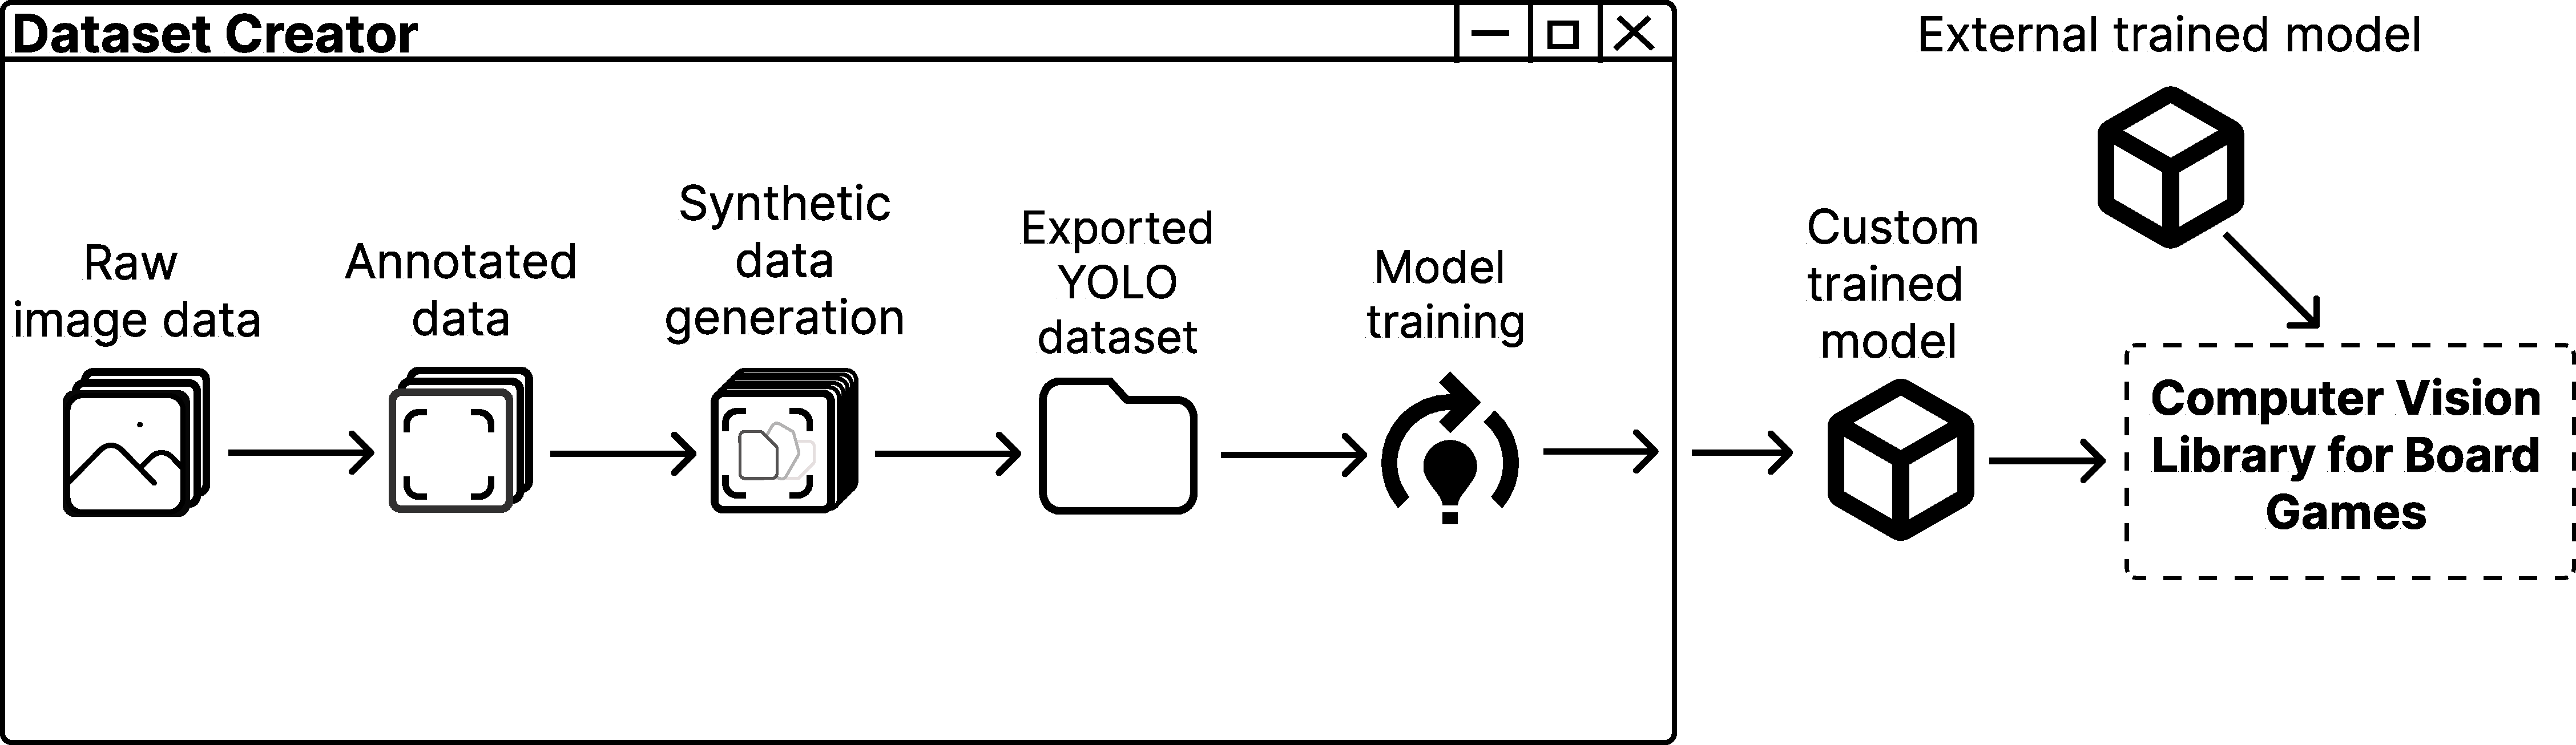
\includegraphics[width=1.0\textwidth]{obrazky-figures/dataset_creator_scheme.pdf}
	\caption{Workflow supported by Dataset Creator for preparing object detection models for CVLiBG.}
	\label{ProjectScheme}
\end{figure}

% =======================================================================================

% =======================================================================================


\section{Used technologies}
The Dataset Creator should be usable by developers on all operating systems, as Android development is not exclusive to a single operating system. Therefore, it is necessary to use cross-platform frameworks. Even though the Dataset Creator is part of this thesis, CVLiBG must be usable independently. Similarly, the Dataset Creator can be used only as an annotation or dataset preparation tool, without using the mobile library. Therefore, all data needed to make datasets must be saved in one of the standard formats, allowing users of the application to convert datasets into other formats using external tools, should they desire to.

\subsection{Python}
There are plenty of options for choosing a library or framework that supports desktop development. Most of these languages support multi-platform development. However, some of them, like C++ would require multiple binaries or building from source. On the other hand, interpreted languages such as Java provide more seamless multi-platform deployment, and the code from the mobile applications could be shared with the desktop dataset application. 

However, while Java has many positives, it is also known to be a verbose language with more code overhead. Python, on the other hand, seems to be more popular for neural networks and object detection in general. 

\subsection{PySide and Qt}
Many modern frameworks support multi-platform development. The list became a bit narrower by choosing Python as the main language. Options such as Kivy, Tkinter, PyQt, PySide, Flet, and many more could be found as fully fledged development frameworks; some of them even support mobile development. 

Qt\footnote{What is Qt: \url{https://wiki.qt.io/About_Qt}} is a multi-platform application development framework for desktop, embedded, and mobile applications. It is supported and used by many companies; however, it was chosen mainly due to having previous experience with this framework, which allowed smoother and faster development of the application.

There are two implementations of Qt for Python: PyQt and PySide. Both of these versions are very similar nowadays, and the main difference comes from who manages the projects. PyQt is managed by Riverbank Computing Ltd.\footnote{PyQt about: \url{https://www.riverbankcomputing.com/software/pyqt/intro}}, while PySide is managed and maintained by The Qt Company\footnote{PySide6, Qt for Python: \url{https://doc.qt.io/qtforpython-6/}}. The most notable difference is licensing. PyQt is available under GPL or commercial license, while PySide uses a more permissive LGPL license\footnote{Licensing differences between PyQt and PySide: \url{https://www.pythonguis.com/faq/pyqt6-vs-pyside6/\#licensing}}. While this project will be open and not used for commercial purposes, the more permissive license is preferred. Therefore, PySide was chosen as the framework for desktop development.

\subsection{OpenCV}
OpenCV was also used in the Dataset Creator for image loading, saving, and manipulation. Its main role is in the synthetic data generation process, where image data is resized, letterboxed, and blurred using OpenCV's methods.

\subsection{Ultralytics}
\label{Ultralytics}
Ultralytics provides pretrained YOLO models under AGPL license. Their official site states that their aim is to make AI easy and accessible to individuals and businesses\footnote{Ultralytics About: \url{https://www.ultralytics.com/about}}, which also aligns with this thesis. Dataset Creator utilizes Ultralytics' YOLO pretrained models as a base, and further trains these models to fine-tune them for a specific board game objects. Ultralytics' Python library also provides ready to use training methods. This all in one solution allows for simplicity during the training of models, which can be further exported into the more versatile Open Neural Network Exchange format (see \ref{chosingInferenceRT}).


% =======================================================================================

% =======================================================================================

\section{Dataset representation and management}
Dataset management represents the first step of the Dataset Creator workflow. In this part of the application, existing datasets can be imported and exported into a suitable format for training with Ultralytics.

\subsection{Importing dataset}
The first step of any dataset is importing data; this can either be annotated or "raw" image data. The responsibility of Dataset Creator is to load these files and make them usable for further processing steps.

Based on the provided root directory, image data with \texttt{.png} and \texttt{.jpg} file extensions will be recursively searched for. Likewise, text files will be searched for. These will be grouped into pairs of image files and text files containing annotations. Files can be separated as long as they have matching file names. All datasets must contain Ultralytics' dataset configuration file name \texttt{data.yaml}\footnote{Object Detection Datasets Overview: \url{https://docs.ultralytics.com/datasets/detect/\#ultralytics-yolo-format}}. 

For existing datasets, application expects the Ultralytics configuration file
\texttt{data.yaml} to be present. For newly created datasets, this file is generated and
managed automatically by Dataset Creator.

This file is also used by the Dataset Creator to translate integer class indexes into strings that are used for annotating.

\subsection{Representation of annotated images}
Imported image and label data are paired into \texttt{ImageSample} objects. These contain the path to the original files, as they are not loaded on import. If this were not the case, memory usage for even relatively small datasets, with only a few hundred image files, could be unmanageable for most personal computers. This approach allows for on-demand loading of image data. 

Image samples also contain a list of \texttt{LabelBox} objects. These represent labels, annotations, or bounding boxes. These simple objects contain coordinates, width, height, and class index of the detection they represent. These are used as the ground truths for training. 

% ===============================================================================

\subsection{Exporting datasets}
\textbf{Exporting} is another part of this application. As mentioned before, Dataset Creator uses the Ultralytics YOLO format and enables synthetic data generation of exported datasets with different options: 

\begin{itemize}
  \item {\textbf{Training data percentage} will set the amount of data used for training, the rest will be used for validation.}
  
  \item {\textbf{Generate name from the class} replaces images and text label names with the string representation of detected class and hash generated from the image. Images with multiple classes will be named \texttt{mix\_hash}. This option is mostly for manual inspection of data and it is not required.}
  
  \item {\textbf{Separate classes into subdirectories} option sorts the images and labels based on their detected class into subdirectories. Images with multiple classes will be placed into a mixed subdirectory.}
  
  \item {\textbf{Generate synthetic data for training} enables generating of synthetic data for the training part of the dataset.}

  \item {\textbf{Generate synthetic data for validation} enables generating of synthetic data for the validation part of the dataset.}
  
  \item {\textbf{Export original image} enables/disables the export of the original image. If this option is disabled, only the generated synthetic data will be exported.}
\end{itemize}

Exporting is a computationally heavy operation, especially when synthetic data are being generated. Therefore, it is necessary to use parallelization of the task, leaving the UI on the main thread and heavy tasks on another; otherwise, the application would just freeze and continue using resources until the job is done. Because of that, Dataset Creator allows users to split this task across more threads using the \textbf{Export worker threads} option.

% ==============================================================================

% ===========================================================================


\section{Image annotation}
Image annotation is one of the main functions of the Dataset Creator. The \textbf{Image labeling} page provides tools for manual and automatic data annotation.

\subsection{Representation of annotated data}
Annotating or labeling image data is done by creating rectangle bounding box-like objects. These objects are called \texttt{ImageLabelBoxes} and are used for the graphical representation of the annotated data. These boxes can be created, moved, resized, or deleted. The colors of these boxes can be configured using color pickers. This should increase visibility based on the image and its background, as well as decrease eye-strain during manual annotation.

This page also contains a view for browsing image samples. Samples can be changed by clicking on a specific sample, using \texttt{Next} and \texttt{Previous} buttons, or with the keyboard shortcuts \texttt{"Q"} and \texttt{"E"}.

Deleting selected boxes is done by pressing the \texttt{Delete label} or by pressing the \texttt{"X"} shortcut on the keyboard. Likewise, creating a new label box can be done with \texttt{"Space"} shortcut or the \texttt{New label} button. 

\subsection{Label classes}
Each label box requires its value; otherwise, it will just be a bounding box without a description. These labels can be chosen from the label browser. This browser contains the index \textit{"\#"} of the label and its name. These values are loaded and saved to the \texttt{data.yaml} file. 

Single click on the label will change the currently selected \texttt{ImageLabelBox}. Double-clicking on the label enables the editing mode in which the user can edit the name of the label. The index of the labels cannot be changed. These labels can be added and deleted using the \texttt{New} and \texttt{Delete} buttons. Deleting one label will update the indexes of all other labels with a higher index to move down.

It should be noted that newly created boxes will be assigned a \texttt{default} or previously selected label value. The \texttt{ImageLabelBoxes} with the \texttt{default} value cannot be saved, and users will be warned with a red background in the image sample browser. 

\subsection{Automatic detection}
Automatic detection is intended to speed up the annotation process. This can be useful when annotating larger datasets. Especially because it switches from manually creating every bounding box to inspecting and correcting already created ones.

However, this functionality also has several limitations. It requires a previously trained model that is compatible with the Dataset Creator, and the quality of the generated annotations depends on the accuracy of that model. Therefore, automatic detection should be treated as an annotation aid rather than a replacement for manual review.

This functionality requires opening the model, loading it, and selecting the threshold value for filtering. Annotation is done per image with \texttt{Detect} button or by pressing the keyboard shortcut \texttt{"Tab"}. 

Automatic detection does not account for already created \texttt{ImageLabelBoxes} in the image sample. Therefore, running automatic detection on an already annotated image may create duplicate or overlapping boxes, which must be checked manually.

The current version of the Dataset Creator supports only ONNX Runtime for YOLO models.

% ==================================================================================

% ==================================================================================

\section{Generating synthetic data}
Object detection models trained on small datasets are prone to \textbf{overfitting} (see~\ref{overfitting}). To increase the dataset's size and improve accuracy, Dataset Creator supports creating synthetic data for the training of neural networks.

\subsection{Filter creation}
The synthetic data are generated during the export process. Therefore, this page does not generate synthetic data; instead, it provides a way to create and edit filters used for the synthetic data generation. An explanation of data augmentation and synthetic data is discussed in Section~\ref{dataAugmentation}. 

Filters can be selected from the list of filters; they can also be created, renamed, or removed. These values are stored in the user settings (the \texttt{settings.json}); therefore, they are movable between projects/datasets.

It should be noted that the synthetic data will be exported as finished images with annotated data, which results in additional data and space required by the dataset. However, this format allows datasets to be used outside of the Dataset Creator and may also result in faster training, as the data will not have to be augmented in memory during training.

\subsection{Customization of synthetic data}
\textbf{Flipping}, as stated in \cite{dataAugmentation1}, is one of the easiest and most intuitive ways to augment the data. Simple vertical and horizontal flipping of images can create three additional images for training. However, using this method for direction sensitive data \cite{dataAugmentation1} such as letters and numbers might result in inaccurate labels and detection.

\textbf{Blur} is also considered a good addition, especially as it removes noise from images introduced by compression methods, lighting environment, and camera processing.

The photometric transformations, such as \textbf{Saturation}, \textbf{Brightness}, and \textbf{Contrast}, can be used to change the representation of colors in image data rather than the position of pixels. Lighting biases are an ongoing problem for object detection tasks; being able to artificially create darker or lighter images in a few steps can help enhance the neural network's adaptability \cite{dataAugmentation2}. Another example would be using saturation to accommodate different types of cameras in smartphones, as not all camera sensors are the same.

\textbf{Noise insertion} consists of injecting or changing pixel values in an image. This method is a very good solution for positional biases \cite{dataAugmentation2}. This method makes neural networks more robust, as real world data is not always perfect and often contains graphical artifacts \cite{dataAugmentation1}. The most common methods are \textbf{Gaussian} and \textbf{Speckle} methods. The \textbf{Gaussian} method is an additive technique that changes the original pixel value by adding or subtracting a value from it. \textbf{Speckle}, also known as Salt and Pepper, is a spike noise method. It changes pixels to their extremes, either white or black, reminiscent of salt and pepper.

\textbf{Resolution-related} settings allow for a decrease in the size of the dataset and may result it faster training, as image will not have to resized during training.

% ===========================================================================================

% ===========================================================================================

\section{Training models in Dataset Creator}
The last part of the Dataset Creator is a training solution based on Ultralytics' python library. This UI based, few click solution is meant for quick and simple training inside the application, using created datasets.

Therefore, for more efficient model training, the developers should seek different solutions.

\subsection{Training options}
This last page allows changing the settings provided to Ultralytics' trainer. The list of options consists of: pretrained model, model path, project name, training epochs, patience, workers, and batch size.

The \textbf{pretrained models} define the backbone and architecture used to create the final fine-tuned model. Available models are Ultralytics' YOLO 8, 11, and 26 versions with three model sizes: Nano, Small, and Medium.

\textbf{Model path} and \textbf{project name} define where the results will be generated and what name will be used for it.

A single \textbf{epoch} represents a complete pass of the model over the entire training dataset. Each epoch ends with an evaluation on the validation part of the dataset.

\textbf{Patience} represents the number of epochs after which training will be ended if no improvements in accuracy are achieved.

\textbf{The} number of additional worker threads used during training is referred to as workers. This value depends on the hardware capabilities of the machine running the application.

\textbf{Batch size} represents the number of training examples in one training pass. Higher values mean higher memory use, which also results in faster training.